%%%%%%%%%%%%%%%%%%%%%%%%%%%%%%%%%%%%%%%%%%%%%%%%%%%%%%%%%%%%%

\mainmatter
\setcounter{page}{1}

\lectureseries[\course]{\course}

\auth[\lecAuth]{Lecturer: \lecAuth\\ Scribe: \scribe}
\date{October 13, 2009}

\setaddress

% the following hack starts the lecture numbering at 6
\setcounter{lecture}{5}
\setcounter{chapter}{5}

\lecture{Frequency Domain Analysis}

\section{Why Use Frequency Domain?}
Recall that the cross-spectral density function is defined as
$$\Phi_{yu}(\w) = \mathcal{F}\{R_{yu}(\tau)\}$$
No information is lost when moving from the time domain to the frequency domain because this is a unitary transformation.

\begin{example}
Apply the input $u(t) = \sum_{k=1}^n Ak\sin(\w_kt+\phi_k)$, where $\phi_k\in\mathcal{U}[0,\pi]$, with $\mathcal{U}$ representing a uniform distribution. What does the spectrum of the signal look like?

There are $n$ $\delta$-functions with amplitude $\frac{Ak}{2\pi}$ such that
$$\Phi_u(\w) = \sum_{k=1}^n \frac{Ak}{2\pi}\delta(\w-\w_k)$$
$\lozenge$
\end{example}

Following that, what happens to the frequency resolution of $\Phi_u(l\cdot\Delta\w)$ as $\lim_{N\to\infty}T = N\dt$? The frequency resolution goes to zero, $\Delta\w\to 0$. This means that the more samples taken the closer the discrete-time representation is to a continuous-time representation. However, since $\Phi_u(\w)$ is a function of $\delta(\w-\w_k)$ the only information that matters is at $\w_k$. This property has several important consequences:
\begin{itemize}
\item Data compression -- $n$ points in the frequency domain represent $N>>n$ points in the time domain.
\item For periodic signals, information at $N$ time domain points is fully represented by $n$ points in the frequency domain. However, this does not work for $\{u(t)\} =$ white noise.
\end{itemize}
In a later lecture we will see how to approximate signals as periodic even when they are not in order to take advantage of these data compression properties.

\begin{lemma}
This is Lemma 2.1 in Ljung. Let $\{s(t)\}$ be a quasi-stationary signal with spectrum $\Phi_s(\w)$. Let $S_N(\w) = \frac{1}{\sqrt{N}} \sum_{t=1}^N s(t)e^{-j\w t}$, with $|t|\in\mathbb{N}$ and $\w\in\mathbb{R}$. Knowing
\begin{align*}
\Phi_s(\w) &= \mathcal{F}\{R_s(\tau)\} \\
\hat{\Phi}_s^N(\w) &= \mathcal{F}\{\hat{R}_S^N(\tau)\} = S_N(\w)S_N^*(\w) = |S_N(\w)|^2
\end{align*}
then the following result holds
$$\lim_{N\to\infty} \fint E\{|S_N(\w)|^2\}\Psi(\w)d\w = \fint \Phi_s(\w)\Psi(\w)d\w$$
where $\Psi(\w)$ is sufficiently smooth.
\end{lemma}
The expected value converges weakly to the spectrum. We need the additional term and the integral to get convergence.

The result of this lemma is bad news. $\hat{\Phi}^N(\w) = \mathcal{F}\{\hat{R}_u^N(\tau)\}$ only converges weakly to the actual spectrum, $\Phi(\w)$. The good news is that, if in addition to the quasi-stationary constraint, the function $\sum_{\tau=0}^\infty|\tau R_s(\tau)|<\infty$ is bounded, then
\begin{itemize}
\item $\lim_{N\to\infty}E\{\hat{\Phi}_s(\w)\} = \Phi_s(\w)$. For this to work $R_s(\tau)$ needs to go to zero faster than $\tau$. See Figure \ref{fig:06autoCovDecay}. This happens automatically if $s(t)=L(q)e(t)$, where $L(q)$ is a BIBO filter and $e(t)$ is white noise.
\item $\lim_{N\to\infty}E\{[\hat{\Phi}_s^N(\w)-\Phi_s(\w)]^2\} = \Phi_s^2(\w)$. The squared term represents the variance, $\sigma$, of the signal and $\sigma$ never goes to zero. This is more bad news.
\item $\lim_{N\to\infty}E\{[\hat{\Phi}_s^N(\w_1)-\Phi_s(\w_1)][\hat{\Phi}_s^N(\w_2)-\Phi_s(\w_2)]\} = 0$. This means that the variance beteween neighboring points goes to zero. This can be used in a way that makes it good news.
\end{itemize}

\begin{figure}[ht!]
	\centering
	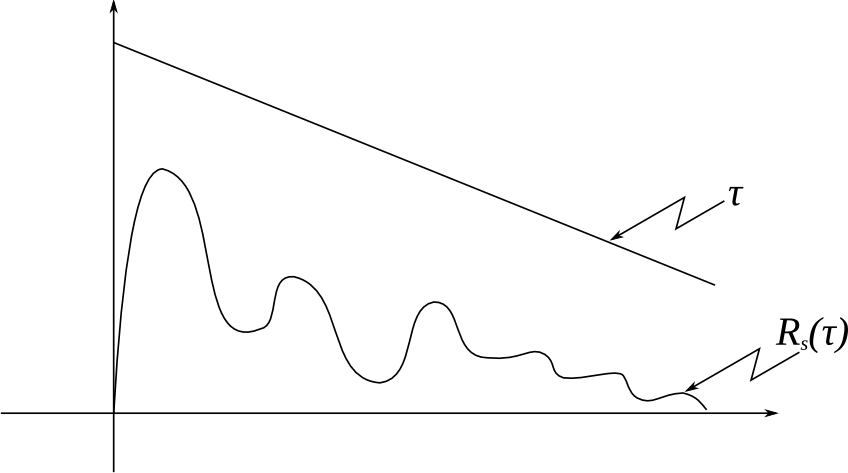
\includegraphics[width=.4\textwidth]{images/06autoCovDecay}
	\caption{Rate of decay of auto-covariance function and $\tau$.}
	\label{fig:06autoCovDecay}
\end{figure}

\begin{example}
\label{ex:sSpectrum}
Try this in \textsc{Matlab}. Let $s(t)=L(q)e(t)$ have $\{e(t)\}$ be white noise and $L(q)$ be a second-order Butterworth filter (see Figure \ref{fig:06butterworthFilter}). What does the spectrum, $\Phi_s(\w)$, look like?
\begin{align*}
\Phi_s(\w) &= \mathcal{F}\{R_s(\tau)\} \\
&= \mathcal{F}\{\bar{E}\{s(t)s(t-\tau)\}\} \\
&= \mathcal{F}\{\bar{E}\{(L(q)e(t))(L(q)e(t-\tau))\}\} \\
&= \mathcal{F}\left\lbrace E\left\lbrace\lim_{N\to\infty}\frac{1}{N}\sum_{t=1}^N(L(q)e(t))(L(q)e(t-\tau))\right\rbrace\right\rbrace \\
&= L(e^{j\w})L^*(e^{j\w})\Phi_e(\w) \\
&= |L(e^{j\w})|^2
\end{align*}
$\lozenge$
\end{example}

\begin{figure}[ht!]
	\centering
	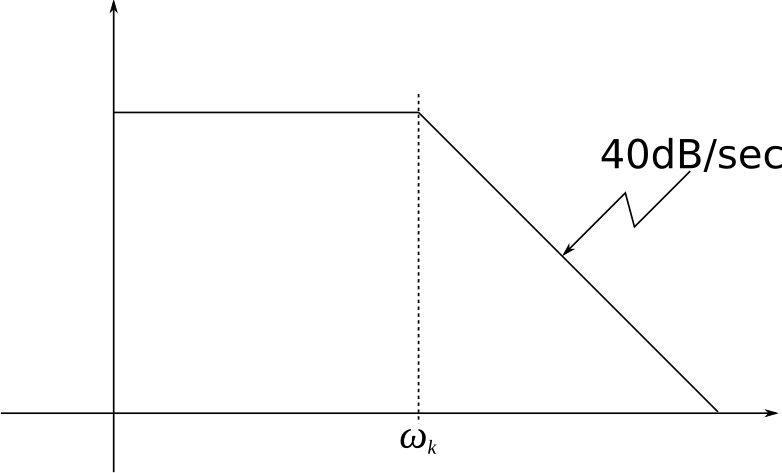
\includegraphics[width=.4\textwidth]{images/06butterworthFilter}
	\caption{Second-order Butterworth filter.}
	\label{fig:06butterworthFilter}
\end{figure}

The response from Example \ref{ex:sSpectrum} looks like Figure \ref{fig:06freqResp}. Note that the estimate will look jagged because of the variance. Also, the x-axis is a log scale so there are more points near $\pi/\dt$. An important feature is that adding more points does not make the variance go to zero. The variance will always be there. However, since the variance betweeen neighboring points goes to zero we have that $\sigma(\w_1)$ has no effect on $\sigma(\w_2)$.

\begin{figure}[ht!]
	\centering
	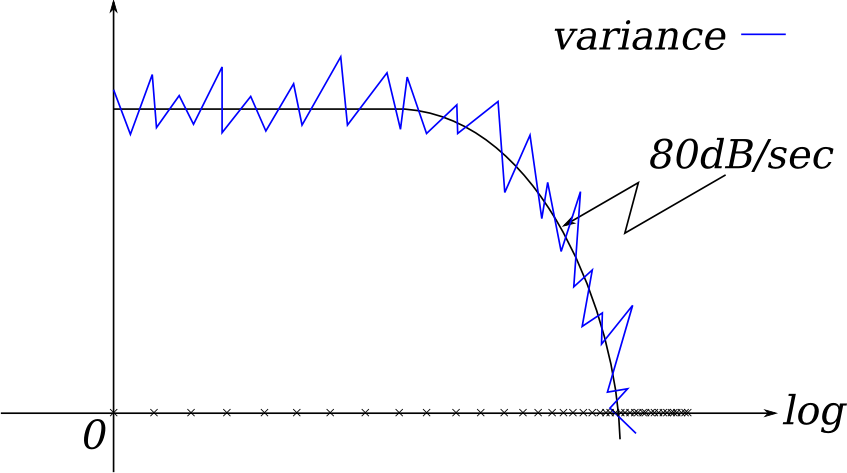
\includegraphics[width=.5\textwidth]{images/06freqResp}
	\caption{Frequency response with variance.}
	\label{fig:06freqResp}
\end{figure}

To reduce the variance we can take the average of the spectrum over a small range. By doing that over the entire spectrum of the signal the effect is that we are multiplying the spectrum by a window function called $w(\w)$, which can also be thought of as a weighting function. The result of using a rectangular window of width $\xi$ is
$$\hat{\hat{\Phi}}_s^N(\w) = \frac{1}{2\pi}\int_{\w=-\pi}^\pi \Phi_s^N(\xi)w(\xi-\w)d\xi$$
When $w(\w)$ is not a simple rectangular window with range $[0,1]$ this estimate must be normalized by dividing the right hand side by $\frac{1}{2\pi}\int_{\w=-\pi}^\pi w(\w)d\w$.

\begin{theorem}
$$\lim_{N\to\infty}\hat{\hat{\Phi}}_s^N(\w) = \Phi_s(\w) \text{ w.p. } 1$$
provided $w(\w)$ is sufficiently smooth.
\end{theorem}
The expression $\text{w.p. } 1$ means that $\sigma\to 0$. The term $\hat{\hat{\Phi}}_s^N(\w)$ is called the spectral estimate, spectral analysis or spectral estimation.

\section{Spectral Analysis}
Spectral analysis is the convolution of the crude estimate $\hat{\Phi}_s^N(\w)$ with $w(\w)$ so that we get $\hat{\hat{\Phi}}_s^N(\w) \to \Phi_s(\w) \text{ w.p. } 1$. Recall that $\hat{\Phi}_s^N(\w) = \mathcal{F}\{R_s(\tau)\} = |S_N(\w)|^2$. This gives
$$\hat{\hat{\Phi}}_s^N(\w) = \mathcal{F}\{R_s(\tau)\} * \mathcal{F}\{w(\tau)\} = \mathcal{F}\{R_s(\tau)\} * w(\w)$$
where the $*$ symbol represents the convolution operator. Taking the inverse Fourier transform yields
$$\mathcal{F}^{-1}\{\hat{\hat{\Phi}}_s^N(\w)\} = \hat{\hat{R}}_s^N(\tau) = \hat{R}_s^N(\tau)\cdot w(\tau)$$
since the inverse Fourier transform of convolution is multiplication. This is referred to as ``windowed estimation'', where $w(\tau)$ is the ``time window'' and $w(\w)$ is the ``frequency window''. Note that using $w(\w)$ being a $\delta$-function would result in no change to the variance because $\mathcal{F}^{-1}\{\delta(\w)\} = 1$. Also, $w(\tau)$ and $w(\w)$ are functions that can be tuned by an engineer and give some flexibility for efficiently averaging out the variance. See Figure \ref{fig:06windowfilter}.

\begin{figure}[ht!]
	\centering
	\subfloat[Frequency window.]{
		\label{fig:06freqWin}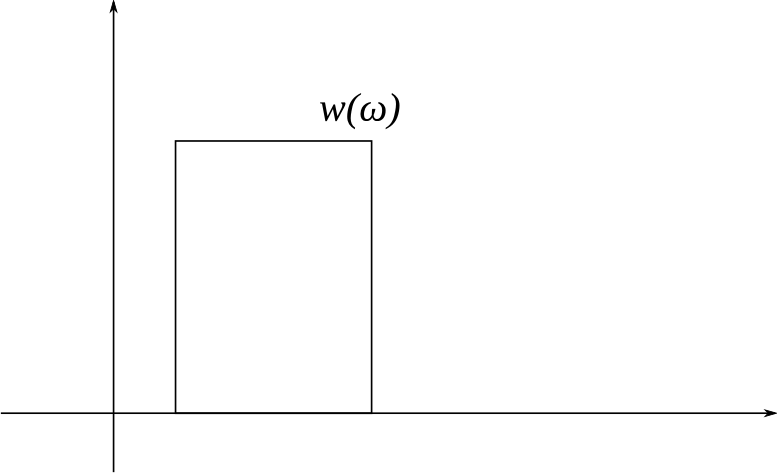
\includegraphics[width=0.4\textwidth]{images/06freqWin}
	} \hfill
	\subfloat[Time window.]{
		\label{fig:06timeWin}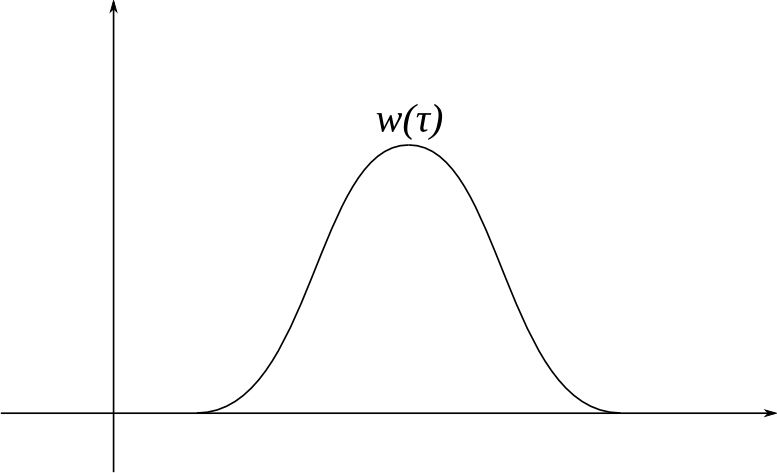
\includegraphics[width=0.4\textwidth]{images/06timeWin}
	}
	\caption{The same window filter in the \subref{fig:06freqWin} frequency domain and the \subref{fig:06timeWin} time domain.}
	\label{fig:06windowfilter}
\end{figure}

Summarizing, the windowing functions involve multiplying $\hat{R}_s^N(\tau)$ with $w(\tau)$ or convolving $\hat{\Phi}_S^N(\w)$ with $w(\w)$, where $w(\w)=\mathcal{F}\{w(\tau)\}$. This windowing operation is essential to obtaining a consistent estimate of the spectrum of a signal.

\subsection{Common Windows}
Some common windows, as specified in the time domain, are listed below. Note that $\gamma$ is the design variable.

\subsubsection{Rectangular Window}
$w_\gamma(\tau) = 1$, with $1<|\tau|\leq\gamma$. See Figure \ref{fig:06rectWin}.

\subsubsection{Bartlett Window}
$1-\frac{\tau}{\gamma} \Leftrightarrow \frac{1}{\gamma}\left(\frac{\sin\gamma\w}{\sin\w}\right)^2$, with the time domain on the left and the frequency domain on the right. See Figure \ref{fig:06bartlettWin}.

\subsubsection{Hamming/Hann Window}
$\frac{1}{2}\left(1+\cos\frac{\pi\tau}{\gamma}\right)$. See Figure \ref{fig:06hammingWin}.

\begin{figure}[ht!]
	\centering
	\subfloat[Rectangular window filter.]{
		\label{fig:06rectWin}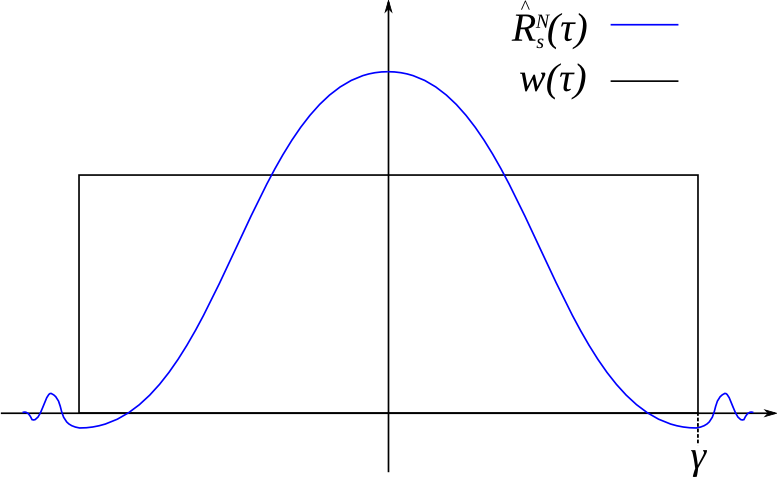
\includegraphics[width=0.4\textwidth]{images/06rectWin}
	} \hfill
	\subfloat[Bartlett window filter.]{
		\label{fig:06bartlettWin}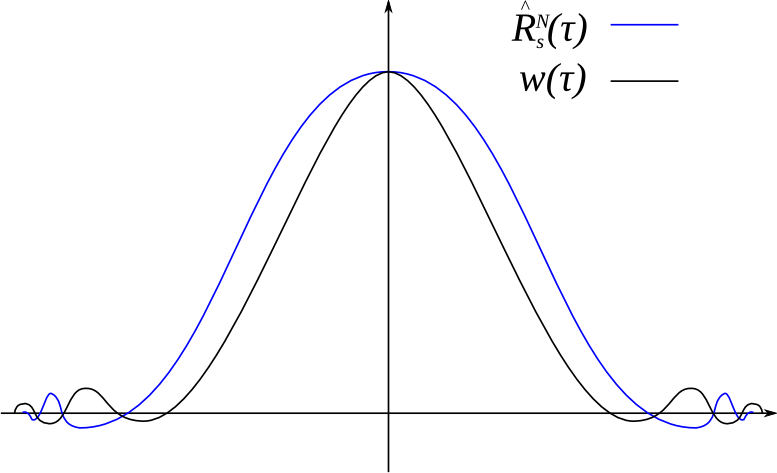
\includegraphics[width=0.4\textwidth]{images/06bartlettWin}
	} \hfill
	\subfloat[Hamming/Hann window filter.]{
		\label{fig:06hammingWin}\includegraphics[width=0.4\textwidth]{images/06hammingWin}
	}
	\caption{Different shapes of window filters.}
	\label{fig:06filterShapes}
\end{figure}

\subsection{Welsh Method}
The Welsh method is another way of averaging to reduce the noise on a spectral estimate, $\hat{\Phi}_s^N(\w)$. The first step is to split the data with $N$ points into $k\cdot N_0$ points as in Figure \ref{fig:06welsh}. Assume $k=8$ for the next steps. Second, compute $\hat{\Phi}_s^{N_0}(\w)$ for each period $k$, $\hat{\Phi}_s^{N_0} = |S_{N_0}(\w)|^2$. Third, calculate
$$\hat{\hat{\Phi}}_s^N(\w) = \sum_{k=1}^8 \hat{\Phi}_s^{N_0}(\w)$$
Then, instead of working with $\bar{E}\{s(t)s(t-\tau)\}$ use
\begin{align*}
\frac{1}{N}\sum_{t=1}^Ns(t)w(t)s(t-\tau)w(t-\tau) =
\frac{1}{N}\sum_{t=1}^Ns(t)s(t-\tau) \underbrace{w(t)w(t-\tau)}_{w(\tau)}
\end{align*}
The Welsh method is similar to the Bartlett window when setting $\gamma=N_0$ in the expression $1-\frac{\tau}{\gamma}$.

\begin{figure}[ht!]
	\centering
	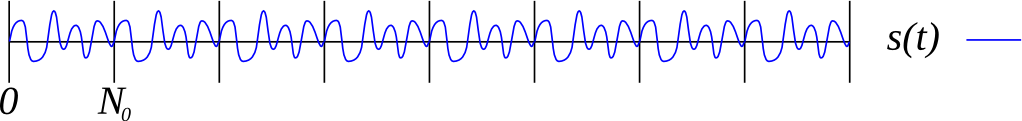
\includegraphics[width=.5\textwidth]{images/06welsh}
	\caption{Welsh window method.}
	\label{fig:06welsh}
\end{figure}

%%%%%%%%%%%%%%%%%%%%%%%%%%%%%%%%%%%%%%%%%%%%%%%%%%%%%%%%%%%%%